%!TEX root = main.tex

\section{Analysis of Voice Recognition Flow}

\subsection{Analysis Framework}

\begin{figure}[th]
\centering
	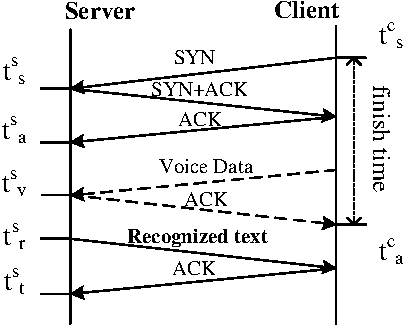
\includegraphics[scale=0.7]{voice_flow_rtt}
\caption{Time-line in voice recognition flow.}
\label{fig:voice_flow_rtt}
\end{figure}

Figure~\ref{fig:voice_flow_rtt} shows the time-line in voice recognition flow. From client side, the finish time is from that client initiates the connection to that client receives all acknowledgments of the voice data, \ie $t^c_a - t^c_s$. From server side, finish time is approximated as $(t^s_v - t^s_s) + (t^s_t - t^s_r)$, where $t^s_v$ is the time that server receives all voice data. As mentioned above, at most 3 RTT's could be measured from server side in voice recognition, including $t^s_a - t^s_s$ and $t^s_t - t^s_r$ in the figure, as well as the RTT when server terminates connection (not shown in the figure).

RTT is ambiguous when the corresponding segment is retransmitted. To investigate the impact of RTT on finish time, we use the following strategy to determine the baseline RTT. If there is no retransmission of SYN packet, $t^s_a - t^s_s$ is used as the RTT of the flow. Otherwise, the RTT when server terminates the connection is used, if the FIN packet is not retransmitted. When both of the two RTT's above are ambiguous, $t^s_t - t^s_r$ is exploited. We have verified in the web search dataset that $t^s_a - t^s_s$ is the minimal RTT in more than 60\% of flows, and is less than 2 times of the minimal RTT in 95\% of flows. Thus it is reasonable to assume that the measured RTT from server side could represent the minimum RTT from client side in voice recognition.

\begin{figure*}[th]
\centering
	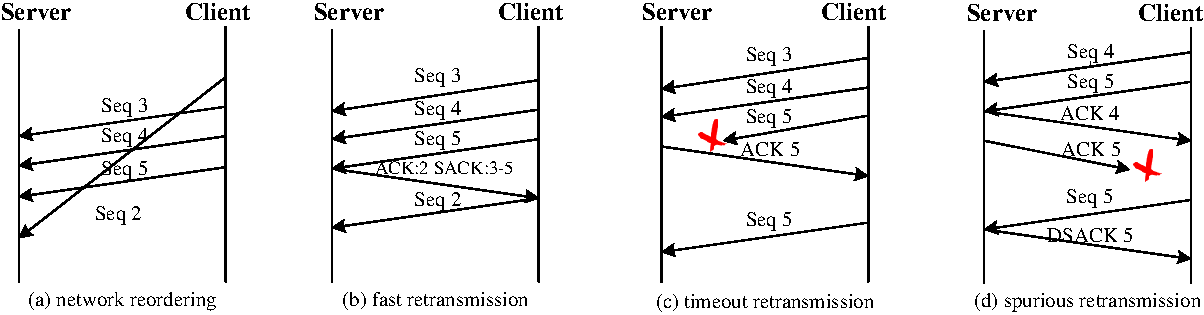
\includegraphics[scale=0.7]{voice_flow_estimate_retrans}
\caption{Server could not distinguish packet loss and reordering in voice recognition.}
\label{fig:voice_flow_estimate_retrans}
\end{figure*}

Figure~\ref{fig:voice_flow_estimate_retrans} exemplifies that server could not distinguish packet loss and reordering when receiving data from client. In Figure~\ref{fig:voice_flow_estimate_retrans}(a), there are packets reordered by network, which could not be distinguished from fast retransmission in Figure~\ref{fig:voice_flow_estimate_retrans}(b). From server side, it could not distinguish whether the packet is retransmitted or reordered by network. In Figure~\ref{fig:voice_flow_estimate_retrans}(c), client retransmitted segment 5 when retransmission timer is triggered. From server side, it could not identify packet loss, but only feels that the interval between segment 4 and segment 5 is long. Server could sense unnecessary retransmission when receiving data packet twice, and notifies the spurious retransmission to client via Duplicate SACK~\cite{rfc3078}, which is shown in Figure~\ref{fig:voice_flow_estimate_retrans}(d).

\subsection{Causal Analysis of Finish Time}

\begin{table}[th]
\centering
\renewcommand{\arraystretch}{1.2}
\caption{Percentage of abnormal flows in different ISP's.}
\label{tab:voice_stats}
\begin{tabular}{l|c|c|c}
	\toprule
	 & CT & CU & CM \\
	\midrule
	packet reordering & 2.3\% & 3.1\% & 4.9\% \\
	\hline
	SYN retransmission & 2.1\% & 1.7\% & 4.5\% \\
	\hline
	timeout retransmission & 5.3\% & 4.9\% & 4.9\% \\
	\hline
	incomplete transmission & 0.2\% & 0.3\% & 2.4\% \\
	\bottomrule
\end{tabular}
\end{table}

Figure~\ref{tab:voice_stats} shows the percentage of abnormal flows in each ISP. A flow is abnormal if it encounters packet loss, reordering, timeout retransmission, or incomplete retransmission. In the table, about 2$\sim$5 percentage of flows are with packet reordering. About 5\% of flows experience timeout retransmission, which is larger than that of flows with packet reordering. The reason is as follows. First, 

Even though the flows are short, with no more than 6 data packets, there are flows 

\begin{table}[th]
\centering
\renewcommand{\arraystretch}{1.2}
\begin{tabular}{l|l|l|l|l|l|l}
	\toprule
	& \multicolumn{3}{c|}{ RTT(s) } & \multicolumn{3}{c}{ reordering (\#(pkts))} \\
	\midrule
	ISP & CT & CU & CM & CT & CU & CM \\
	\midrule
	wifi & 0.1 & 0.088 & 0.198 & 0.026 & 0.034 & 0.056 \\
	\hline
	2G & 0.062 & 0.029 & 0.07 & 0.079 & 0.046 & 0.057 \\
	\hline
	3G & 0.039 & 0.025 & 0.052 & 0.078 & 0.038 & 0.069 \\
	\hline
	4G & - & - & 0.05 & - & - & 0.01 \\
	\bottomrule
\end{tabular}
\caption{The average RTT and number of disordered packets for each access type.}
\label{tab:voice_access_type_stats}
\end{table}


\begin{table}[th]
\centering
\renewcommand{\arraystretch}{1.2}
\begin{tabular}{l|m{.35in}|m{.35in}|m{.35in}}
	\toprule
	& CT & CU & CM \\
	\midrule
	$[$ 0.04, 0.08 ) & 1.50 & 1.60 & 1.52 \\
	\hline
	$[$ 0.08, 0.12 ) & 1.83 & 2.69 & 1.97 \\
	\hline
	$[$ 0.12, 0.16 ) & 2.76 & 3.22 & 3.23 \\
	\hline
	$[$ 0.16, 0.20 ) & 3.72 & 5.40 & 8.06 \\
	\hline
	$[$ 0.20, $\infty$ ) & 13.2 & 25.6 & 29.2 \\
	\bottomrule
\end{tabular}
\caption{}
\label{tab:}
\end{table}

\begin{table}[th]
\centering
\renewcommand{\arraystretch}{1.2}
\begin{tabular}{l|c|c|c}
	\toprule
	ISP & CT & CU & CM \\
	\midrule
	PCC & 0.0002 & 0.002 & -0.003 \\
	\bottomrule
\end{tabular}
\caption{The Pearson Correlation Coefficients between $finish\_time$ and flow size.}
\label{tab:fin_vs_pkt}
\end{table}

In this section, we investigate how the factor(s) impact the performance in voice recognition. First, we use PCC to inspect the relationship between $finish\_time$ and flow size in the three ISP's. The correlation coefficients are shown in Table~\ref{tab:fin_vs_pkt}. From the table, the $finish\_time$ of flows is completely irrelevant to the flow size. The reason is as follows. Most of flows contain no more than 6 data packets, which could be packed in the initial congestion window from client side.

% TODO explain the reason why flows in CU experience such a high transmission time.
\begin{figure}[!htbp]
\centering
	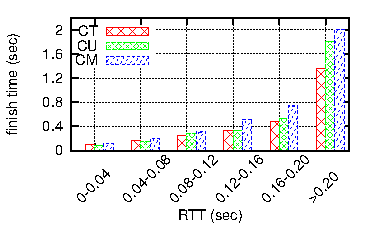
\includegraphics[width=3in]{voice_rtt}
\caption{The finish time under various RTT's in voice recognition.}
\label{fig:voice_rtt}
\end{figure}

Next, we study the impact of RTT on the $finish\_time$ in voice recognition. The RTT's are measured according to the strategy in Section~\ref{sec:dataset}. We group the flows into different bins by their RTT's, with 0.04 second intervals. Figure~\ref{fig:voice_rtt} plots the average $finish\_time$ of flows in each bin. From the figure, as the RTT value becomes larger, the finish time increases correspondingly. When the RTT value is less than 0.20 second, finish time has a roughly linear relationship with RTT. In fact, the correlation coefficients between the mean value of finish time in each bin and the index are more than 0.83, 0.81, 0.85 in the three ISP's. In the figure, the ratio of average finish time to the RTT value falls in the interval $[2, 4]$, except that when RTT value is larger than 0.2 second. When the RTT value is larger than 0.2 second (corresponding to 8\% of flows), the average finish time is more than 1.2 second. The reason is as follows. Larger RTT indicates that the packets are buffered in the network for longer time, which is also a signal of network congestion, like in TCP Vegas\cite{brakmo1995tcp}, FastTCP\cite{wei2006fast}. Thus when flow experiences large RTT, it is likely that the flow is traversing congested network, and may encounter packet loss, thus has exceptional large finish time.

\begin{figure}[th]
\centering
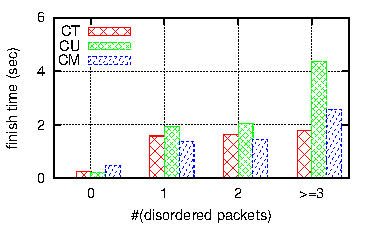
\includegraphics[width=3in]{voice_reorder}
\caption{The finish time under different number of disordered packets in voice recognition.}
\label{fig:voice_reorder}
\end{figure}

In the above, we have analyzed that from server side, packet loss and reordering could not be distinguished. In the following, we will take packet reordering as an indication of network congestion and study the impact of network congestion on finish time. In packet reordering, the number of disordered packets is defined as follows. In receiving sequence $S_2, S_4, S_5, S_3$, the packet $S_3$ is disordered, thus the number of disordered packets is 1. Figure~\ref{fig:voice_reorder} shows the average finish time under different number of disordered packets. From the figure, in all three ISP's, when there are disordered packets, flows experience significant performance degradation.

Even when there is only 1 disordered packet, the average finish time is 2$\sim$8 times higher than that of flows without disordered packet. This could be explained as follows. If server receives packets which are not successive, it feeds back to the client with SACK. When receiving SACK, client does not retransmit the packet in the hole (\ie the disordered packet) immediately, until client receives 3 SACK's or ACK of that packet, or retransmission timer is triggered. If the packet is dropped, client needs to wait at least one RTT to retransmit the packet. If there are not sufficient number of SACK's, client has to rely on timeout retransmission (RTO). The RTO timer, as an estimate of the RTT and variation in RTT, is usually highly conservative, which is set to tens of, or even hundreds of RTT. Especially in CU, when flows have more than 2 disordered packets, the average finish time is 20 times higher than that of flows without packet reordering.

The significant impact of network congestion on finish time motivates us to investigate the impact of timeout retransmission on finish time in voice recognition. We use the following trick to identify each RTO. For each packet, there is an estimated arrival time, calculated according to the time of preceding and subsequent packets. If the gap between actual arrival time and the estimated arrival time is larger than $max(200ms, 3 RTT)$, it is identified as a RTO.

As there are no more than 6 data packets in most of voice recognition flows, if there are 3 or more packets dropped, client has to rely on RTO to recover the transmission. 

% Figure~\ref{fig:voice_rto} 

\subsection{Summary of Voice Recognition Analysis}